\chapter{8. Conclusions and Future Work}

This final chapter concludes the thesis and summarizes the main conclusions and presents a number of thoughts on future work.

The Persuasive Electric Vehicle was conceived to be an \textbf{alternative to the car in urban transportation}. This vehicle, along with other strategies, will progressively take the cars out of the urban areas. The PEV finds itself between the bike and the car. Its weight, size and price makes it very attractive for city councils who are willing to reduce pollution and congestion from their cities. As a vehicle of the future, it combines the three main concepts of the future of transportation: \textbf{electrification, autonomy an shared economy}.

It is important to highlight that this thesis vehicle had the purpose of \textbf{experimenting with an active tilting system}, which accounts for the principal innovation in lightweight vehicles like PEV. Other active systems, like the rear propulsion, the steering and the haptic feedback in the handle bar were additions to complete the active control of all the motions in the vehicle. 

Furthermore, the vehicle was designed with a very clear idea in mind: it vehicle had to be \textbf{easy to ride for any user}, independent of their age and experience with bicycles, for example. In fact the design and dimensions of the PEV do were thought to not restrict the handling of the vehicle to any user.

This project has focused on the stability of the PEV and from a general perspective, on the \textbf{stability and balance of lightweight three wheeler vehicles}. However, the PEV is addressing more issues that the ones related with stability. The autonomy package is upgrading day by day thanks to the improvement in the computational power and price of embedded systems like NVIDIA Jetson TX2. In this way, this vehicle will be completed with the autonomous package that Changing Places group is developing.

\newpage
Thanks to the group's \textbf{modular component philosophy}, the design on the vehicle allows the embodiment of the sensors of the autonomous package (LIDAR, ultrasound sensors and stereo-camera) in the frame of the vehicle. Not to mention that the existing electronics in this vehicle --composed of the two Arduino Megas and the rest of controllers and sensors-- can be integrated into the embedded Jetson TX2 by means of the ROS environment in Linux.

Regarding the \textbf{research goals} outlined at the beginning of the thesis, the main objective was to design and fabricate a three wheeler vehicle with an incorporated active tilting system. It can be concluded that the main goal of this thesis was overall achieved, but it has to be pointed out that the fact that tests with driver were not performed does not fully complete it. However, the proposed solutions agree with the existing constraints due to the size, the weight and the cost of a lightweight vehicle like PEV.

The \textbf{selection of the motors and the mechanical components} was adequate for the limitations of the vehicle. Specifically, regarding the tilting motor, the attached planetary gears were ideal for increasing the output torque, which is the main limitation with Direct Tilting Control systems. This prevented any problem to tilt the vehicle in the curves and to maintain it in the vertical position when standing.


After reviewing the current developments in vehicle modeling, roll control and tire modeling, a \textbf{tilting control system} was implemented in the fabricated vehicle. The justification for the selection of DTC rather than STC lays in the range of speeds of the PEV and also in the complexity of the solutions. In this way, the previous work in the field of tilting vehicles cleared the view and showed the limitations and problems of the applied techniques.

Uncertainties such as neglected dynamics or environmental factors were overcome by an stability and a robustness analysis of the control strategy. In fact, these \textbf{uncertainties affected the experimental results} as well as the vehicle modeling and simulation. 

The vehicle was set up to \textbf{test the tilting system} and the rest of the active systems. Even though the results were satisfactory, it was not possible to compare the experimental data with the simulations, due to the lack of tests. In other terms, the tilting mechanism and the design of the front suspension probed to be suitable for the vehicle.

Regarding the \textbf{future improvements in the control strategy}, the modeling of the PEV could be improved with real measurements rather than by trusting a computer generated 3D model. The robustness of the control strategy could also improve if the control gains could be calculated in real time based on the signals coming from the vehicle.

\newpage
\[\]
\begin{figure}[!b]
	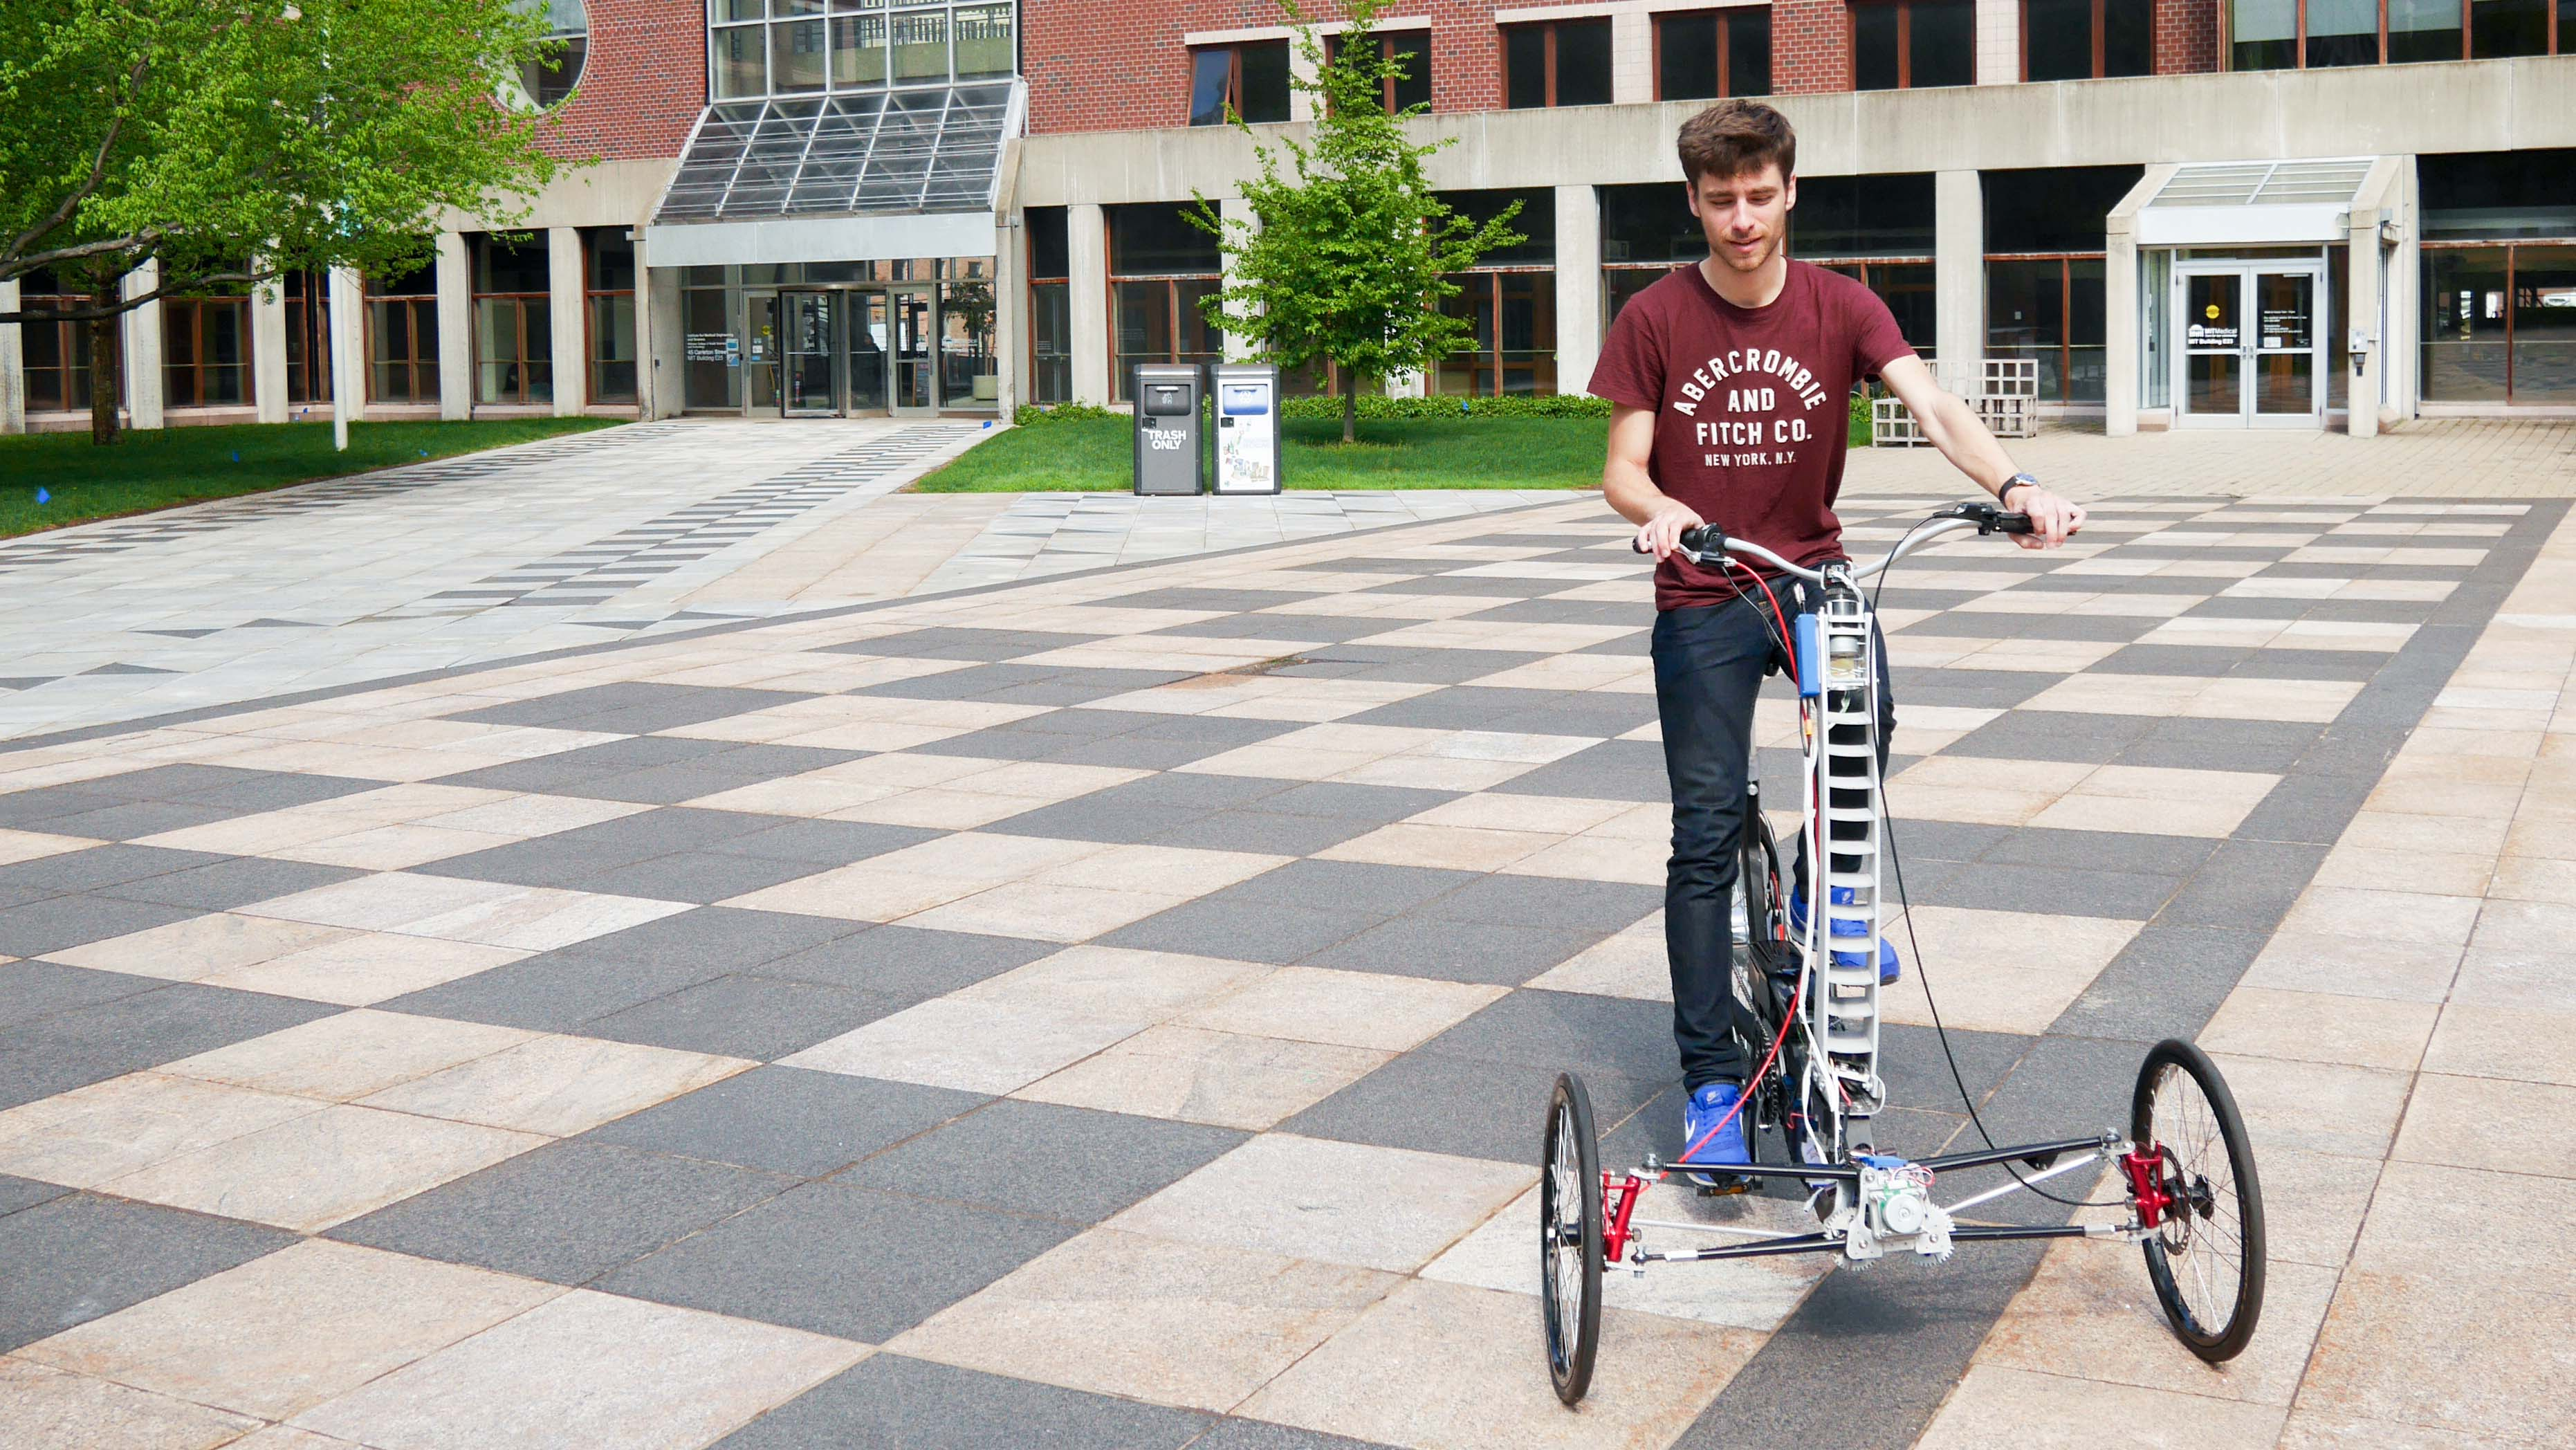
\includegraphics[width=1\linewidth]{figs/06/test_3}
	\caption{Mens et manus}
\end{figure}
